%----------------------------------------------------------------%
%--------------------------INFORMATIONEN-------------------------%
%----------------------------------------------------------------%
%	Infos gibt es zu jedem Paket auf www.ctan.org
%	Werden bei den Paketen bestimmte Optionen gesetzt, so sind die Wichtigsten erklaert
%	solange sie nicht selbsterklärend sind

%----------------------------------------------------------------%
%--------------------------GRUNDEINSTELLUNGEN--------------------%
%----------------------------------------------------------------%
\documentclass[11pt, oneside, ngerman, footinclude=off, captions=tableheading, DIV=12, headerinclude=false, headings=optiontohead]{scrartcl}
\usepackage[bottom=2.5cm, inner=2.5cm, outer=2.5cm, top=2.5cm]{geometry}
%	'oneside'/'twoside': nicht zwischen linker und rechter Seite unterscheiden (alternativ twoside)
%	'twocolumn': wuerde 2 Spalten auf dem Blatt platzieren
%	'bibliography=totocnumbered': Normal nummeriertes Inhaltsverzeichnis (Kapitelnummer)
%	'listof=totocnumbered': Abbildungs- und Tabellenverzeichnis normal nummeriert (Kapitelnummer)
%	'ngerman' verwendet deutsch als Dokumentensprache (z.B. fuer Sirange)
%	'footinclude=off': Zaehlt Fusszeile zum Rand (vergroessert den Textbereich)
%	'captions=tableheading': Tabellenueberschriften explizit verwenden, erhoeht den Abstand zur Tabelle
%	'DIV=12': Kleinere Seitenraender (s. hierzu die KOMA-Documentation)

\usepackage[ngerman, english]{babel}							%	Einstellen der Sprache
\usepackage[T1]{fontenc}							%	Wie wird Text ausgegeben, d.h. im PDF
\usepackage[utf8]{inputenc}							%	Welche Zeichen 'versteht' LaTeX bei der Eingabe?
%\usepackage{lmodern}								%	Laedt Schriften, die geglaettet sind
\usepackage{helvet}     % Helvetica laden (Arial-Ersatz)
\renewcommand{\familydefault}{\sfdefault} % S			
			
											
\usepackage{blindtext}								%	Beispieltext, zum Testen geeignet
%\usepackage{showframe}
%----------------------------------------------------------------%
%--------------------------ABSTÄNDE------------------------------%
%----------------------------------------------------------------%
\usepackage[singlespacing]{setspace}				%	Für Zeilenabstaende: 'singlespacing' (einfach), 'onehalfspacing' (1.5-fach), 'doublespacing' (2fach)
%\setlength{\parindent}{0cm}						%	Laengenangabe für die Einrueckung der ersten Zeile eines neuen Absatzes.
%\setlength{\parskip}{6pt plus 3pt minus 3pt}		%	Laengenangabe für den Abstand zwischen zwei Absaetzen.
%	Wenn diese beiden Befehle nicht kommentiert sind, wird ein Absatz nicht eingezogen sondern es gibt einen Abstand

%----------------------------------------------------------------%
%--------------------------MATHE---------------------------------%
%----------------------------------------------------------------%
\usepackage[]{mathtools}							%	Erweiterung von AMSMath, laedt automatisch AMSMath - für viele Mathe-Werkzeuge, 'fleqn' als Option ist für Mathe linksbuendig
\usepackage{amsfonts}								%	Für eine Vielzahl an mathematischen Symbolen

%----------------------------------------------------------------%
%--------------------------KOPF- UND FUSSZEILEN------------------%
%----------------------------------------------------------------%
\usepackage[automark,headsepline=.4pt]{scrlayer-scrpage}
\pagestyle{scrheadings}
\setkomafont{pageheadfoot}{\normalfont\bfseries}	%	Normale Schriftart und Fett für den Seitenkopf
\addtokomafont{pagenumber}{\normalfont\bfseries}	%	Normale Schriftart und Fett für die Seitenzahl

\clearscrheadfoot
\ohead{\thepage}									%	Rechter Seitenkopf mit Seitenzahl
\ihead{\headmark}									%	Linker Seitenkopf mit section
\ofoot[]{\empty}
%\ofoot{\thepage}									%	Leere Fußzeile, ungerade Seiten
%	Definert man oben in der documentclass 'twoside', so wird zwischen geraden und ungeraden Seiten unterschieden (NUR DANN!)

%----------------------------------------------------------------%
%--------------------------BILDER--------------------------------%
%----------------------------------------------------------------%
\usepackage{graphicx}									%	Um Bilder einbinden zu koennen 
\usepackage[dvipsnames,svgnames,table]{xcolor}			%	Farben verwenden, Versch. Farbdefinitionen, Farben in Tabellen (-Reihen, -Spalten)
\usepackage{pdfpages}									%	pdfs importieren
\definecolor{Seeblau100}{RGB}{0,169,224}				%	Uni-Farben, z.B. fuer Tabellen
\definecolor{Seeblau65}{RGB}{89,199,254}
\definecolor{Seeblau35}{RGB}{165,224,254}
\definecolor{Seeblau20}{RGB}{203,237,254}
\definecolor{Seegrau60}{RGB}{102,102,102}
\definecolor{Seegrau40}{RGB}{153,153,153}
\definecolor{Seegrau20}{RGB}{204,204,204}
\definecolor{Seegrau10}{RGB}{230,230,230}

%----------------------------------------------------------------%
%--------------------------POSITIONIERUNG------------------------%
%----------------------------------------------------------------%
\usepackage{float}

%----------------------------------------------------------------%
%--------------------------LISTEN--------------------------------%
%----------------------------------------------------------------%
\usepackage{enumitem}							%	Um Listen / Aufzaehlungen leichter zu modifizieren
%\setlist{noitemsep}							%	Verringert den Abstand in Aufzaehlungen

%----------------------------------------------------------------%
%--------TABELLEN-/BILDUNTERSCHRIFTEN und NUMMERIERUNG-----------%
%----------------------------------------------------------------%
\addtokomafont{captionlabel}{\bfseries}			%	Abbildung X.Y wir fett geschrieben
\setcapindent{2em}								%	2. Zeile teilweise haengend und eingezogen. Wenn ganz haengend gewuenscht, auskommentieren

\numberwithin{equation}{section}				%	Nummerierung der Gleichungen, Tabellen und Bilder nach der Kapitelnummer
\numberwithin{figure}{section}
\numberwithin{table}{section}

%----------------------------------------------------------------%
%--------------------------LITERATURVERZEICHNIS------------------%
%----------------------------------------------------------------%
\usepackage[german]{babelbib}					%	Bereitstellung des deutschen Layouts fuer die Bibliography

%----------------------------------------------------------------%
%--------------------------SIUNITX-------------------------------%
%----------------------------------------------------------------%
\usepackage[]{siunitx}
\sisetup{locale = DE}							%	Automatische Einstellung der Ausgabe für bestimmte Regionen (UK, US, DE, FR, ZA)

%----------------------------------------------------------------%
%--------------------------URLs / REFs---------------------------%
%----------------------------------------------------------------%
\usepackage[hidelinks]{hyperref}				%	Erweiterte Referenzierung ('hidelinks' verhindert Linien um Links)

%----------------------------------------------------------------%
%--------------------------EIGENE BEFEHLE------------------------%
%----------------------------------------------------------------%
\usepackage{mhchem}
%\usepackage{subfig}
\usepackage{subcaption}
\usepackage{listings}
%\lstset{numbers=none}
\definecolor{backcolour}{rgb}{0.95,0.95,0.92}
%\lstset{
%	numbers=none,
%	language=HTML,
%	breaklines=true,
%	frame=single,
%	tabsize=2,
	%backgroundcolor=\color{backcolour},  
%}

%\lstset{
%  language=HTML,
%  basicstyle=\ttfamily\small,
%  keywordstyle=\color{blue},
%  stringstyle=\color{red},
%  commentstyle=\color{green!50!black},
%  showstringspaces=false,
%  breaklines=true,
%  frame=single
%}

\definecolor{lightgray}{rgb}{.9,.9,.9}
\definecolor{darkgray}{rgb}{.4,.4,.4}
\definecolor{purple}{rgb}{0.65, 0.12, 0.82}

\lstdefinelanguage{JavaScript}{
  keywords={typeof, new, true, false, catch, function, return, null, catch, switch, var, if, in, while, do, else, case, break},
  keywordstyle=\color{blue}\bfseries,
  ndkeywords={class, export, boolean, throw, implements, import, this},
  ndkeywordstyle=\color{darkgray}\bfseries,
  identifierstyle=\color{black},
  sensitive=false,
  comment=[l]{//},
  morecomment=[s]{/*}{*/},
  commentstyle=\color{purple}\ttfamily,
  stringstyle=\color{red}\ttfamily,
  morestring=[b]',
  morestring=[b]"
}

\lstset{
   language=JavaScript,
   backgroundcolor=\color{lightgray},
   extendedchars=true,
   basicstyle=\footnotesize\ttfamily,
   showstringspaces=false,
   showspaces=false,
   numbers=left,
   numberstyle=\footnotesize,
   numbersep=9pt,
   tabsize=2,
   breaklines=true,
   showtabs=false,
   captionpos=b
}


\usepackage{makecell}


\begin{document}
	%---------------------------------------------------------------------------------------------%
	%------------------------------------------TITELSEITE-----------------------------------------%
	%---------------------------------------------------------------------------------------------%
	\title{Project}
	\subtitle{AI in Transportation}
	\author{Author: Johanna Schaefer}
	\date{17.10.2025}
	\maketitle
	\vspace{3cm}
	\pagenumbering{alph}	% Griechische (unsichtbare) Seitenzahlen, damit kein doppeltes Vorkommen
	
	\thispagestyle{empty}	% Seite ohne Seitenkopf
	
	\section*{Abstract}
	This work investigates the use of different machine learning models to predict traffic flow and speed based on sensor data collected from highway portals.
	The main aim is to evaluate and compare two sensor groups to see which can best compensate for a failing sensor: one using data from the same portal and another using data from neighbouring portals. 
	Both, the summed flow for the upcoming 15 minutes and the mean speed, were predicted.
	The secondary objective was to evaluate and compare different model types for this forecasting task. Linear Regression, XGBoost, and Feedforward Neural Networks were investigated. Among these, XGBoost achieved the best overall performance, also allowing a robust NaN-value handling and good training times.
	The results indicate that the flow at the target sensor can be better predicted with the sensors from the neighbouring portal, while for the speed it is better to use sensors from the same portal.
	
	

	
	
	
	\thispagestyle{empty}
	\cleardoublepage
	\thispagestyle{empty}




	\newpage
	%---------------------------------------------------------------------------------------------%
	%------------------------------------------INHALTSVERZEICHNIS---------------------------------%
	%---------------------------------------------------------------------------------------------%
	\tableofcontents
	\thispagestyle{empty}	% Seite ohne Seitenkopf

	\newpage
	\pagenumbering{arabic}	% Arabische Seitenzahlen
	\setcounter{page}{1}	% Seitenzahle auf 1 Setzen
	

	%---------------------------------------------------------------------------------------------%
	%------------------------------------------DOKUMENTENKÖRPER-----------------------------------%
	%---------------------------------------------------------------------------------------------%
	\section{Introduction}
	In modern transport systems, continuous collection of traffic data is essential for providing real-time information on speed and traffic flow. Sensors on road portals provide important data, but individual sensors can fail temporarily. The central question of this work is therefore: To what extent can missing sensors be compensated for by data from other sensors in the same portal or from neighbouring portals?
	To answer this question, a regression approach is used in which the measured values of a target sensor are predicted on the basis of neighbouring sensors. The study examines whether sensors within the same portal provide better prediction accuracy than sensors from a neighbouring portal. 
	The work combines descriptive analysis, feature engineering, and four machine learning methods, including linear models, XGBoost, and neural networks, to develop a deeper understanding of data relationships and prediction potential.
	
	\section{Descriptive analysis}
	\subsection{Data description}
	The data set used for this project consists of speed and traffic flow data from several sensors on the motorway near Stockholm. The data comes from 29 sensors belonging to 8 different portals on a section heading south. Every sensor measures the speed and flow in one line of the motorway. There are inflows and outflows within this section between the portals as can be seen in the illustration in the project instructions.
%	\begin{figure}[H]
%		\centering
%		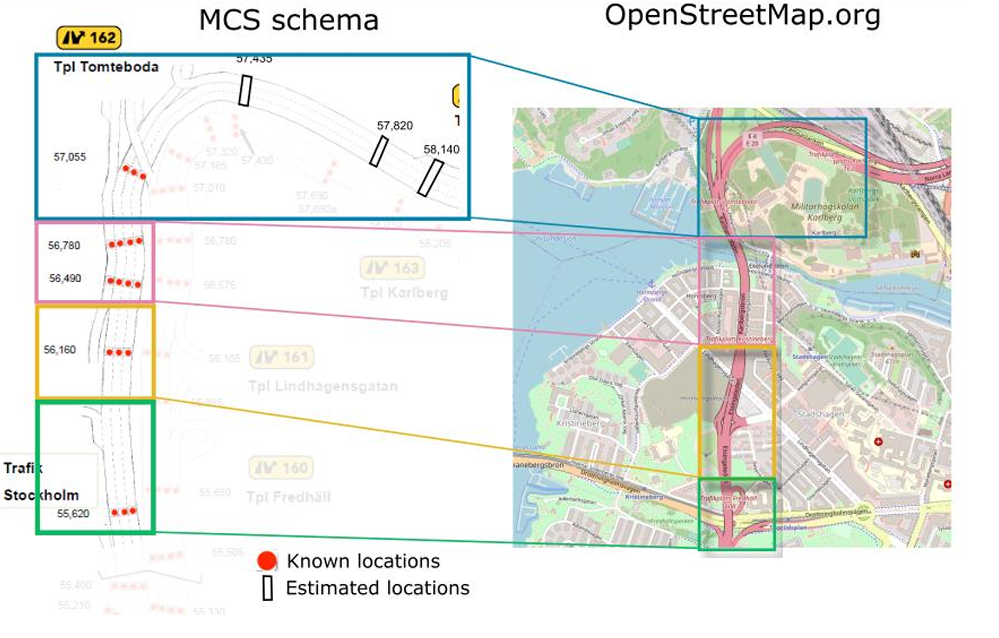
\includegraphics[width=0.7\linewidth]{screenshots/overview}
%		\caption{Overview motorway section and portals}
%		\label{fig:overview}
%	\end{figure}
%	\noindent Table \ref{tab:portalsandsensors} shows the portals and the correspondings sensors.
	\noindent Over a total of 214 days, speed and flow data were recorder between 4 AM and 10 AM with a temporal resolution of one minute.
	Speed is measured in meters per second, while flow is quantified as the number of vehicles per minute.
	\subsection{Speed and Flow per portal}
	Between 4 AM and 10 AM, the flow of vehicles shows a generally increasing trend (see figure \ref{fig:speed_and_flow_overday}), indicating a continued build up of traffic volume as the morning progresses. The rate at which it is increasing is slowing down when approaching the 10 AM mark. In contrast, the average speed tends to decline over the same period, reflecting growing congestion.
		\begin{figure}[H]
		\centering
		\begin{subfigure}{0.49 \linewidth}
			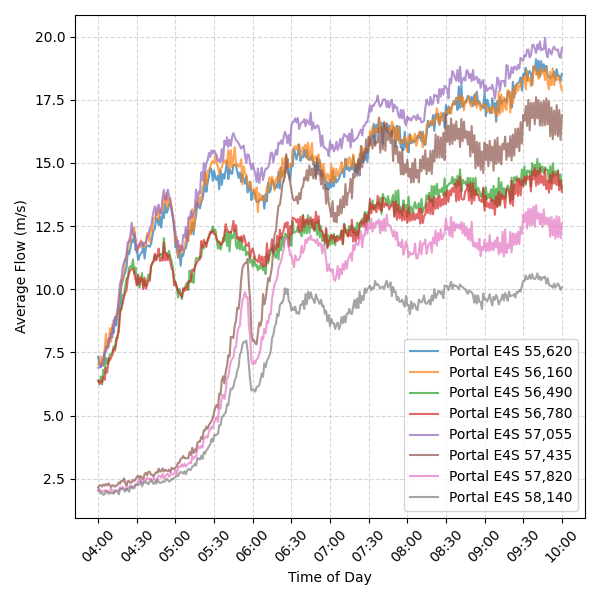
\includegraphics[width=\textwidth]{../Plots/Flow/flow_comparison_portals}
			\caption{Flow}
		\end{subfigure}
		\begin{subfigure}{0.49 \linewidth}
			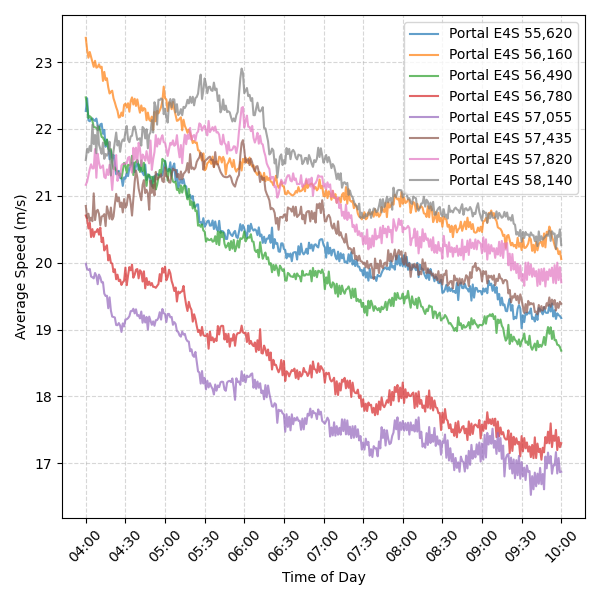
\includegraphics[width=\textwidth]{../Plots/Speed/speed_comparison_portals}
			\caption{Speed}
		\end{subfigure}
		\caption{Flow and Speed over the day in the different portals }
		\label{fig:speed_and_flow_portals}
	\end{figure}
	\noindent This inverse relationship between flow and speed is characteristic of peak-hour dynamics, where higher vehicle density leads to reduced travel speeds.
	Furthermore, it can be seen that it seems like there are two different groups of portals. Portal 55620, 56160, 56490, 56780 and 57055 are more similar to each other than to the other three, which also seem to form a group. \newline 
	\noindent Furthermore, a daily profil on the sensor level can also be created. It can be seen that different sensors within the same portal show different patterns. An example for portal 55620 and 56160 can be found in figure \ref{fig:speed_and_flow_sensors}.
	
	
	
	\subsection{Correlation}
	Furthermore, the correlation between different sensors was analysed for both speed and flow. It is important to note that no time lag was considered in this initial assessment although the time lag also plays a significant role: %In addition to variations in speed and flow across sensors, spatial separation plays a significant role:
	the greater the distance between sensors, the more pronounced the temporal offset and divergence in observed traffic patterns. \newline 
	In figure \ref{fig:sensor_corr_by_portal} the sensors are displayed grouped by the portals they are part of. The thicker black lines indicate the portals.
	\begin{figure}[H]
		\centering
		\begin{subfigure}{0.49 \linewidth}
			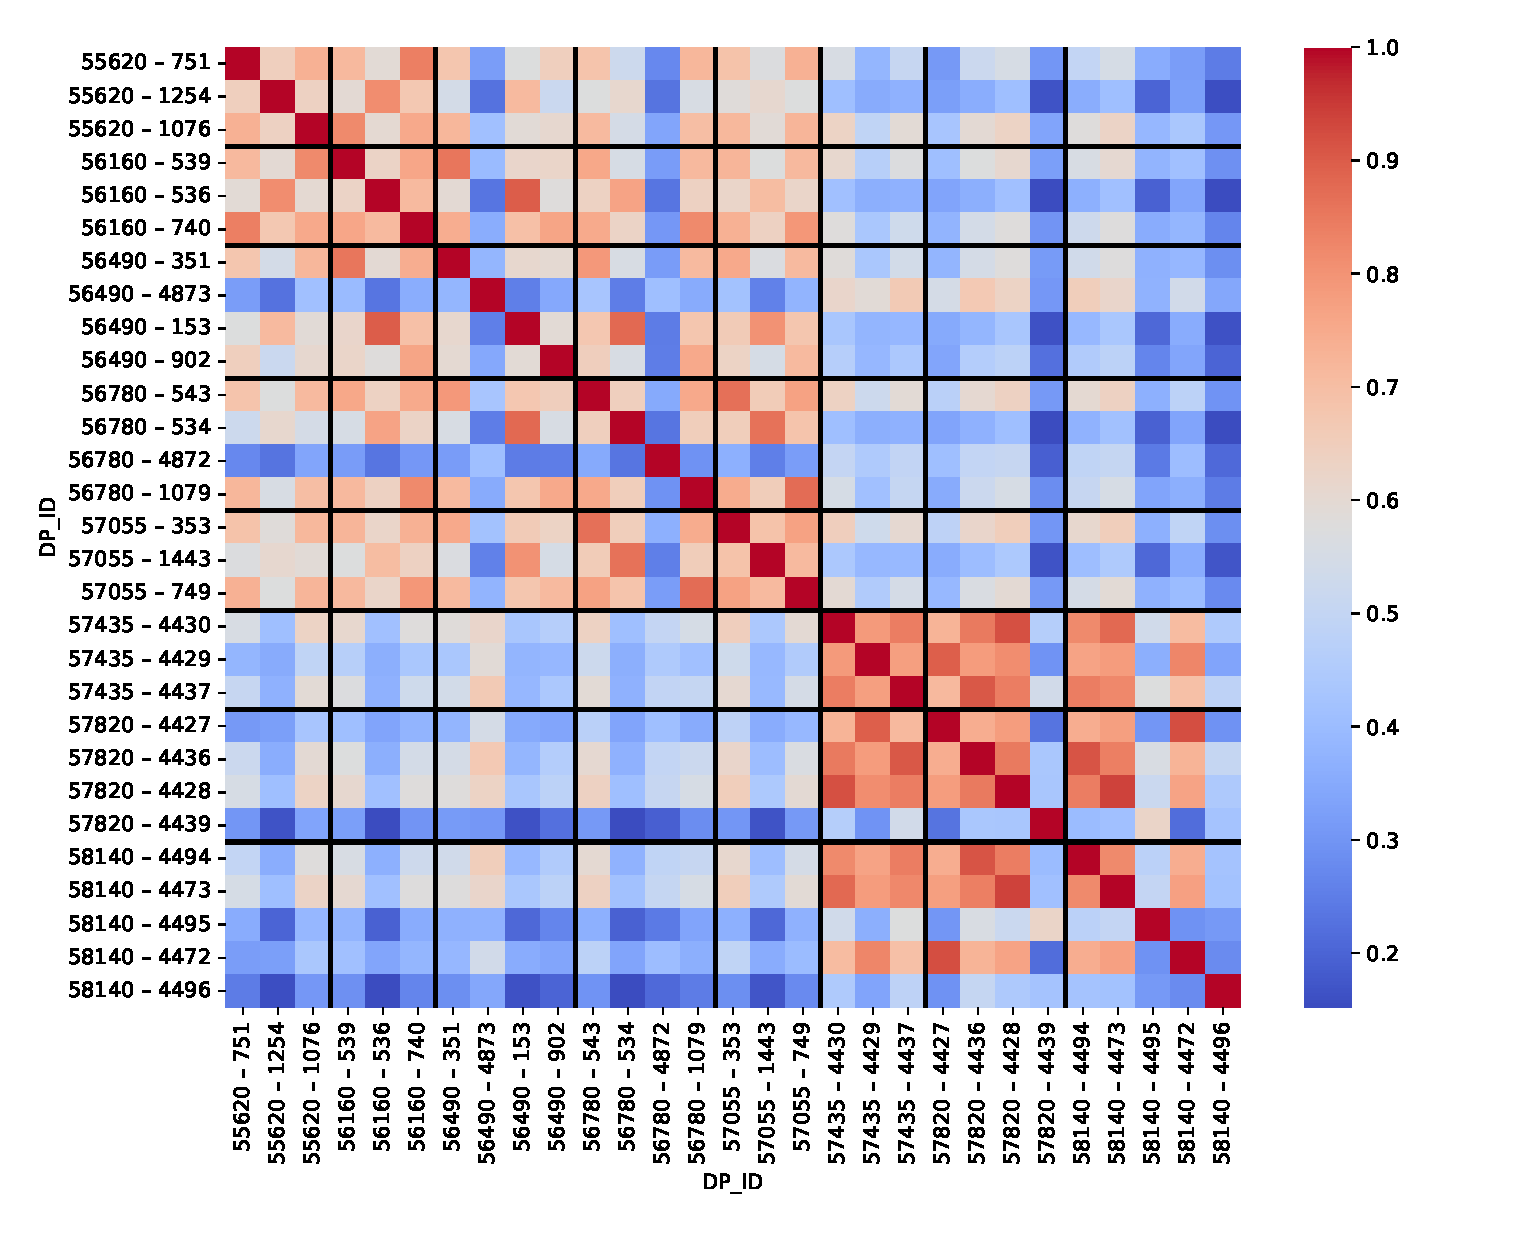
\includegraphics[width=\textwidth]{../Plots/Flow/sensor_corr_by_portal}
			\caption{Flow}
		\end{subfigure}
		\begin{subfigure}{0.49 \linewidth}
			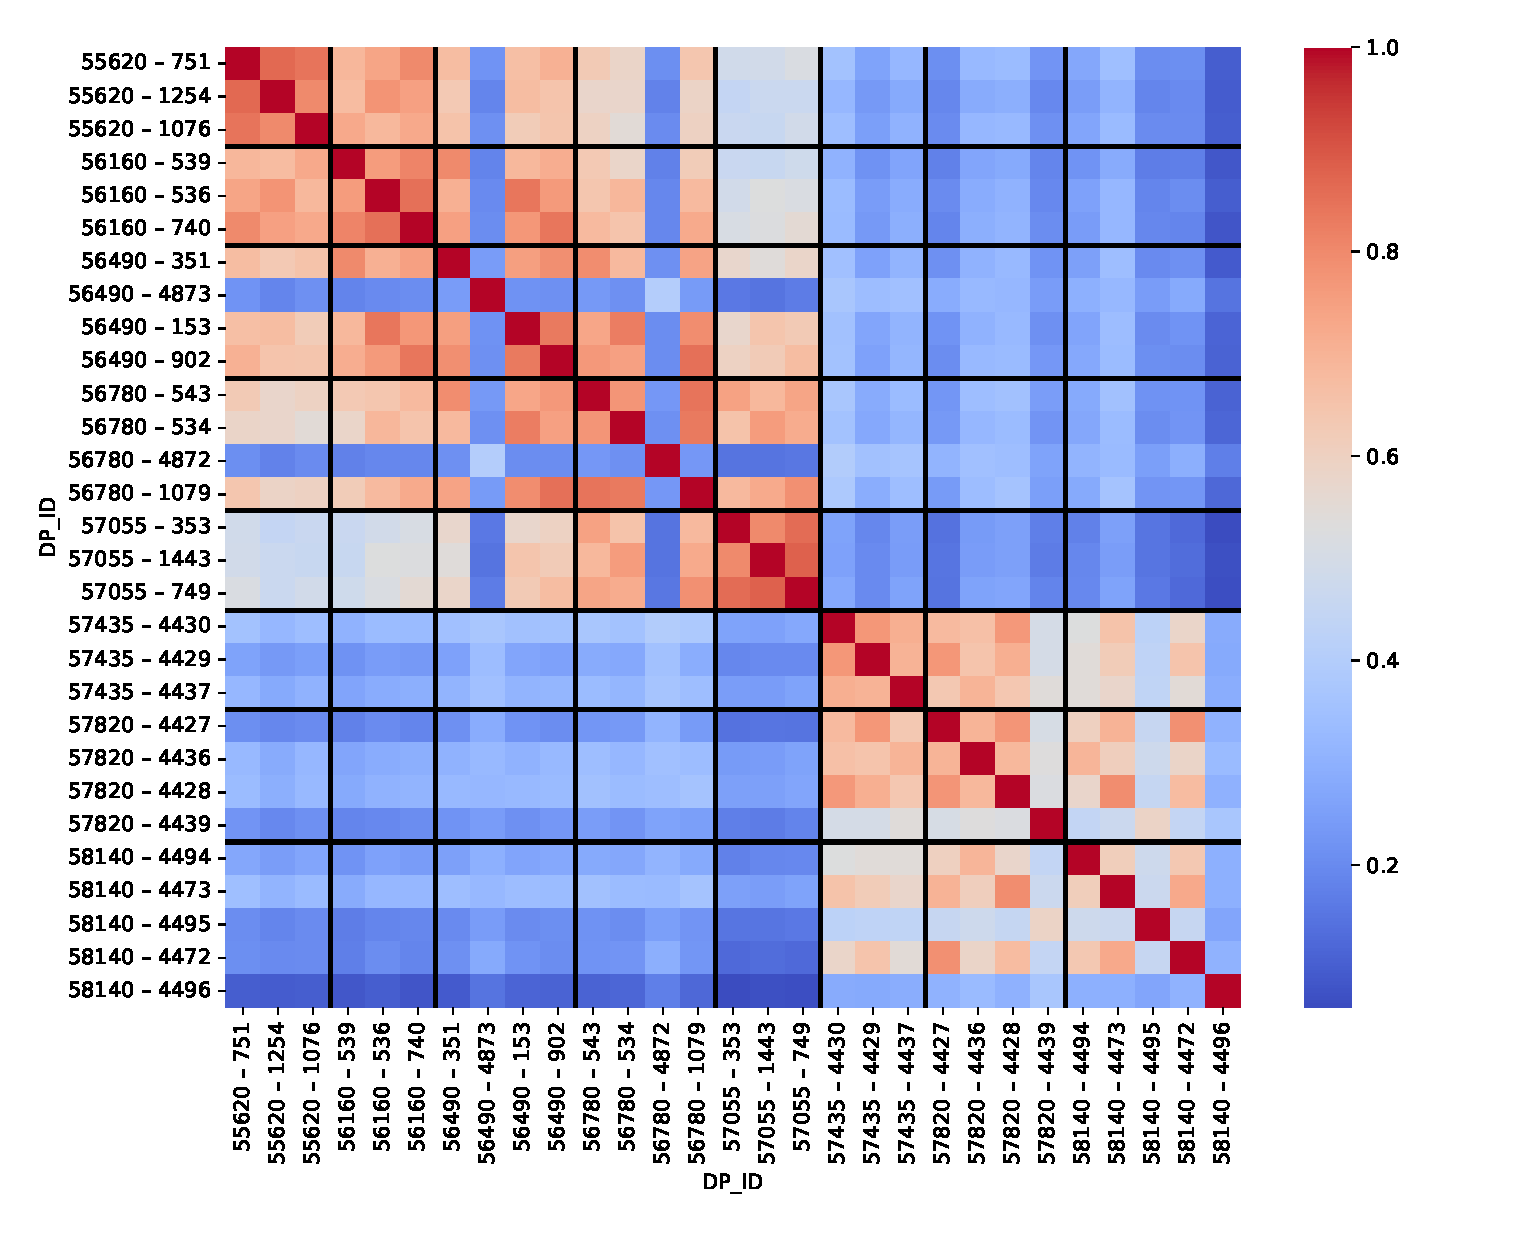
\includegraphics[width=\textwidth]{../Plots/Speed/sensor_corr_by_portal}
			\caption{Speed}
		\end{subfigure}
		\caption{Correlation between speed and flow in different sensors -- the illustration can be found in a bigger format in the appendix \ref{fig:sensor_corr_by_portal_big}}
		\label{fig:sensor_corr_by_portal}
	\end{figure}
	\noindent The two different groups of portals can also be identified in this correlation matrix.
	Furthermore, speed and flow show different patterns. It can be seen that for the speed the correlation is generally higher within the same portal (indicated by high density of red squares close to the diagonal). On the other side, this is not necessarily the case for the flow values. It can be seen that the red squares are more spread out, showing that the correlation is also partially high with sensor data from other portals.
	\subsection{Clustering as lane identification} \label{chap:clustering}
	As part of the data analysis, lane identification was performed using unsupervised clustering.
	The underlying assumption is that different lanes exhibit distinct traffic characteristics in terms of speed and flow. Typically, faster lanes are located on the left (e.g., overtaking lanes), while slower lanes are positioned on the right (e.g., exit or merging lanes). It was hoped to find these behaviour patterns in the sensor data to infer lane structure.
	To uncover these lane characteristics, K-Means clustering was used. It was chosen among several other clustering methods as it is the easiest method to control the number of clusters which should -- in the best case -- represent the lanes.
	Based on the pattern that was observed in the correlation matrix showing two different portals groups, they were clustered separately. \newline 
	For the five portals, the number of clusters was set to 4 according to the number of lanes.
	The clustering was very successful in the sense that each portal has only one sensor per cluster as can be seen in table \ref{tab:cluster}, which suggests that the cluster lane identification approach is appropriate. 
	\noindent Figure \ref{fig:clustering_5portals} shows the typical day profil for the different clusters that were identified.
	\begin{figure}[H]
		\centering
		\begin{subfigure}{0.49 \linewidth}
			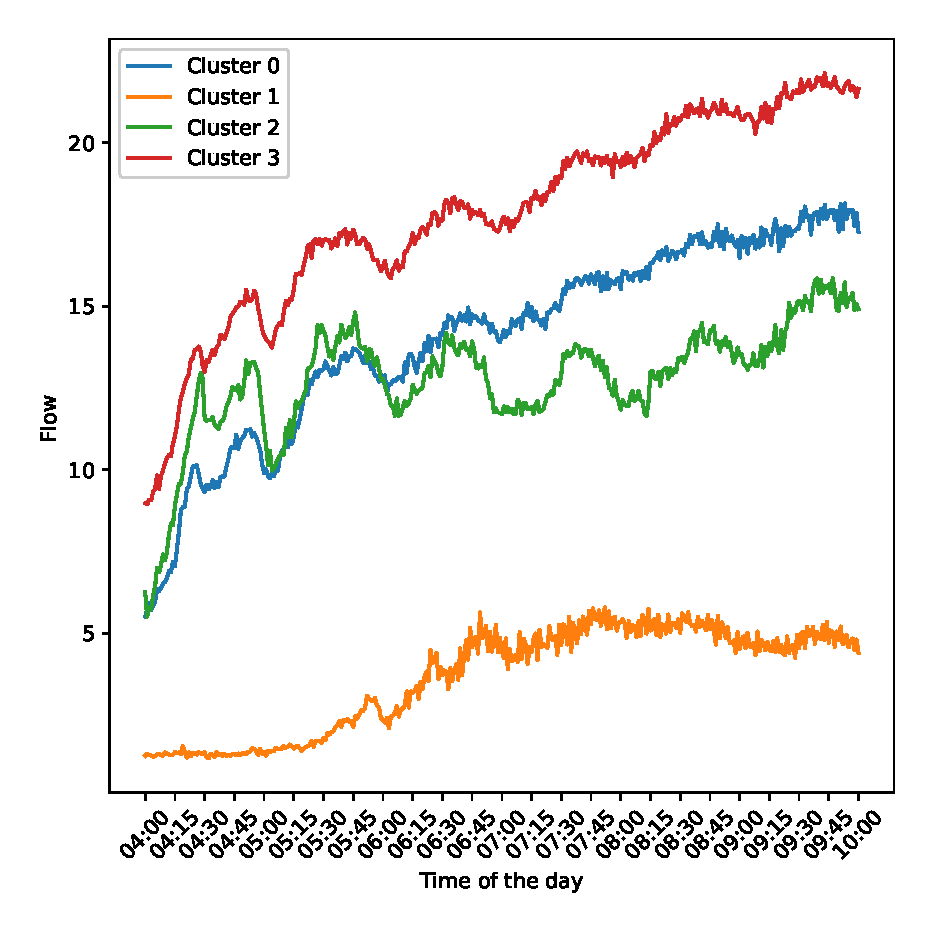
\includegraphics[width=\textwidth]{../Plots/Flow/clustering_5portals}
			\caption{Flow}
		\end{subfigure}
		\begin{subfigure}{0.49 \linewidth}
			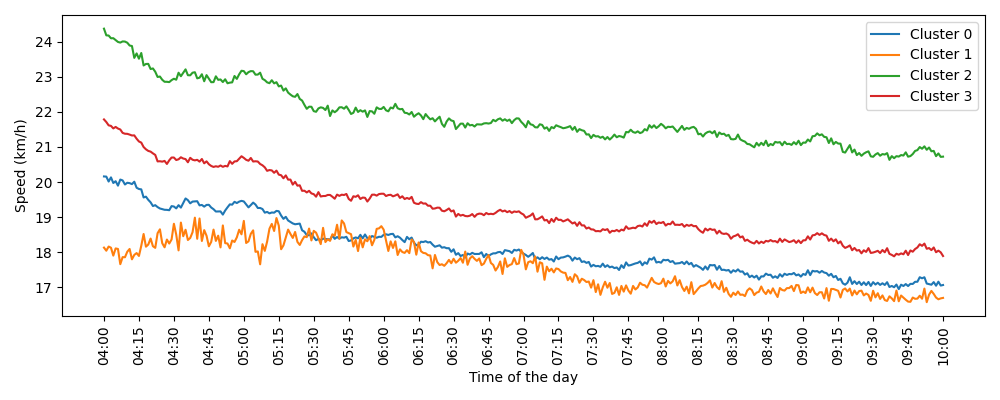
\includegraphics[width=\textwidth]{../Plots/Speed/clustering_5portals}
			\caption{Speed}
		\end{subfigure}
		\caption{Flow and Speed profile of the 4 distinct clusters}
		\label{fig:clustering_5portals}
	\end{figure}
	\noindent Based on these patterns it is very likely -- though not proven -- that cluster 2 corresponds to the leftest lane showing the highest speed, cluster 3 corresponds to the middle lane with a lower speed, cluster 0 the right lane and cluster 1 to the lane where cars enter and leave the motorway with the lowest flow. \newline 
	The clustering for the three other sensors can be found in the appendix \ref{fig:clustering_3portals}.

	\section{Problem formulation}
	The primary objective of this project is to evaluate how well missing sensors can be compensated by using data from other sensors. \newline 
	In real-life traffic management system rely heavily on the data from sensors. However, sensors may fail due to maintenance or technical failure. Thus, it becomes crucial to predict data for the sensors using data from nearby sensors. \newline 
	In this study, the prediction problem is formulated as a regression task, where the target variable represents either the average speed or the summed flow over a future 15-minute interval. The models are trained to predict this value based on lagged features from other sensors.\newline 
	Concretely, the analysis focuses on one reference sensor (Sensor 1076 in Portal 55620). Its values are predicted using two distinct data sources: (1) the two other sensors within the same portal (Sensors 751 and 1254) and (2) the three sensors from the neighboring portal (Sensors 539, 536, and 740). Comparing the predictive performance between these two groups allows for assessing how effectively missing sensors can be replaced by spatially close sensors. In a further step, also portal 57055 is taking into consideration allowing to evaluate the influence of the distance of the neighbouring portal.
	\subsection{Hypothesis}
	The hypothesis of this study is that sensors located within the same portal provide better predictive power for a target sensor than sensors from a neighboring portal.
	\section{Methodology and evaluation methods}
	\subsection{Data preprocessing} \label{chap:dataprepro}
	The raw dataset presented inconsistencies and missing values that necessitated preprocessing.
	The Datetime column was converted to a proper datetime format to allow time-based operations and sequence creation. The \texttt{PORTAL} column was cleaned and standardized in \texttt{PORTAL\_clean} to ensure consistent portal identifiers across sensors.\newline 
	As for the research question of this project only the data of portal 55620,56160 and 57055 was needed, only this data was extracted for further processing. \newline 
	As can be seen in figure \ref{fig:missingvalues} some speed and/or flow values are missing in the dataset for some sensors. Since models like Linear Regression cannot handle NaN values, these missing entries were imputed using forward and backward fill to ensure a complete dataset for modelling.
	%This approach was chosen because traffic conditions tend to change gradually, so using the last known value (forward fill) or the next available value (backward fill) provides a reasonable approximation without introducing abrupt discontinuities.\newline 
	\subsection{Feature engineering}
	To be able to predict the summed flow and average speed at the target sensor, the features had to be chosen. Past values of speed and flow from the same and neighbouring sensors were used as lagged features.
	To justify the number of selected lagged observations, lag correlation  plots were generated for both speed and flow of the target sensor with the lagged observation at the other sensors:
	Figure \ref{fig:correlation_lag} shows that the speed shows a clear transition from a steep to a flat correlation curve at lag $\approx  15$, with a secondary drop at lag $\approx 25$.
	In the flow graph, on the other hand, no clear break is apparent.
	Considering the trade-off betweeen gaining more information and complexity, it was finally chosen to take 15 lagged features for both flow and speed.

	\noindent After selecting the lagged features (past 15 observations for speed and flow), the dataset was transformed into a structured format suitable for model training. Each row of the new dataframe corresponds to a single time point and contains all lagged observations from the relevant sensors as input features (X), while the target variable (y) corresponds to the average speed or summed flow for the next 15-minute interval. 
	\subsection{Model development}
	Several machine learning models were developed to predict the two target variables. The goal was to compare classical regression approaches with more advanced algorithms, including gradient boosting and neural networks, and to evaluate their performance under the same experimental setup.
	For the linear regression model, XGBoost and Feedforward Neural Network a random train-test split was applied, while a simple chronological split was used in the case of LSTM. The data was scaled with a Standard Scaler in the case of the two deep learning models.
	\subsubsection{Linear Regression Model}
	Linear regression was chosen as a baseline model due to its simplicity and interpretability. The model predicts the target variable (either average speed or summed flow) as a linear combination of the lagged features from the same or neighboring sensors.
	\subsubsection{XGBoost}
	XGBoost is a machine learning model that combines many small decision trees. Each tree learns from the mistakes of the previous trees, so that the predictions gradually improve, minimising the squared error as loss function \cite{xgboost_loss}.  It can also handle missing values better and is often more robust against outliers.
	To optimize the performance of the XGBoost model, a Randomized Search \cite{randomsearch} was performed to find the best combination of hyperparameters. The following parameters \cite{xgboostparameters} were considered and adjusted during the search:
	\begin{itemize}
		\item \texttt{n\_estimators}: Number of boosting rounds (trees). A higher number of trees is equivalent to a higher training time and risk for overfitting
		\item \texttt{max\_depth}: Maximum depth of a single tree, controlling model complexity, smaller trees reduce overfitting but can also lead to underfitting.
		\item \texttt{learning\_rate}: Step size shrinkage used to prevent overfitting. Higher values speed up learning but increase the risk of overshooting minima, while smaller values require more trees for the same performance.
		\item \texttt{subsample}: Fraction of training samples used for each tree, lower values reduce overfitting, but increase variance, potentially making predictions less stable.
		\item  \texttt{colsample\_bytree}:Fraction of features used for each tree. Less features reduce overfitting, but might omit important information if set too low.	
	\end{itemize}
	The Randomized Search was performed on the training data only, using 3-fold cross-validation.
	The best model was selected based on the lowest root mean squared error (RMSE) from the cross-validation results.
	\subsubsection{Feedforward Neural Network (FNN)}
	This type of model consists of multiple fully connected layers \cite{book_aicourse}. In an FNN, information flows in one direction only, from the input layer through the hidden layers to the output layer. Each neuron applies a weighted sum of its inputs, adds a bias term, and passes the result through a nonlinear activation function.  The weights are adjusted according to an optimiser, in this case the Adam optimiser.
	Before training, all input features were standardized using a StandardScaler to ensure that all variables contributed equally to the learning process and to improve convergence.
	Each model was trained for up to 100 epochs with a batch size of 32, using mean squared error (MSE) as the loss function and root mean squared error (RMSE) as the evaluation metric.
	Early stopping was applied with a patience of 5 epochs to prevent overfitting, while the learning rate was dynamically reduced when the validation error plateaued.
	In a Gridsearch the number of neurons per layer, the number of layers and the drop out rate were changed.
	\subsubsection{Long Short-Term Memory Network (LSTM)}
	Lastly, an LSTM model was tried out. This is a special neural network that can process time-dependent data and was thus considered relevant for this project \cite{lstm_explanation}. Unlike simple networks, an LSTM can remember previous information and thus can often better capture temporal relationships \cite{differencefnnlstm}.\newline 
	Similar to the FNN, the Adam optimiser was also used and MSE served as loss function while RMSE was used as evaluation metric. tanh was used as activation function.
	In this project two different versions of an LSTM were tried out:
	\paragraph{LSTM with 15 output values:}
	The model gives 15 separate output values for the upcoming 15 minutes. After that, these 15 values are summed up in the case of the flow or averaged in the case of the speed.
	\paragraph{LSTM with one aggregated output value:}
	The model gives one output value which already corresponds to the aggregated value (either summed flow or averaged speed).
	\subsection{Model evaluation}
	To evaluate the performance of the regression models, three error metrics were applied:
	\paragraph{Mean Squared Error (MAE):}
	The Mean Absolute Error measures the average magnitude of the prediction errors. A lower MAE indicates better performance.
	\begin{align}
		\text{MAE}=\frac{1}{n}\sum_{i=1}^{n}\vert y_i-\hat{y}_i\vert
	\end{align}
	\paragraph{Root Mean Squared Error (RMSE):}
	RMSE, compared to MAE, emphasizes larger errors, which is useful when large prediction mistakes are particularly undesirable. A lower RMSE indicates better performance.
	\begin{align}
		\text{RMSE}=\sqrt{\frac{1}{n}\sum_{i=1}^{n}\left( y_i-\hat{y}_i \right)^2}
	\end{align}
	\paragraph{Coefficence of Determination R²:}
	The coefficient of determination (R²) describes how much of the variance in the target variable is explained by the model. An $R^2$
	value close to 1 indicates that the model explains most of the variance, whereas values near 0 indicate weak explanatory power. R² allows for intuitive comparison also across speed and flow that have different units.
	\begin{align}
		R^2=1- \frac{\sum_{i=1}^{n}\left( y_i-\hat{y}_i \right)^2}{\sum_{i=1}^{n}\left( y_i-\overline{y}_i \right)^2}
	\end{align}
	
	\section{Results and Analysis}
	\subsection{Linear Regression}
	As shown in Table \ref{tab:result_linear}, the linear regression model provides a baseline for both flow and speed prediction.
	For the flow the prediction is better using the neighbouring portal with better RMSE, MAE and R² scores, while for the speed the opposite is the case. 
	Furthermore, the R² score indicates that the flow can in general be better predicted than the speed. 
	However, overall performance remains limited which can be seen in the rather low R²-score.
	\begin{table}[H]
		\centering
		\caption{Results obtained with linear regression on test set}
		\label{tab:result_linear}
		\begin{tabular}{l|lll}
			& RMSE   & MAE    & R²    \\
			\hline 
			Flow - same portal      & 33.543 & 23.809 & 0.836 \\
			Flow - neighbour portal & 28.474 & 19.559 & 0.882 \\
			Speed - same portal     & 0.861  & 0.462  & 0.709 \\
			Speed -neighbour portal & 1.051  & 0.513  & 0.566
		\end{tabular}
	\end{table}
	\subsection{XGBoost}
	The XGBoost model (see table \ref{tab:result_xgb}) significantly improves prediction performance compared to linear regression across all cases. This improvement can be attributed to XGBoost's ability to model non-linear relationships between features.
	Again, the neighbouring portal performs better in all metrics for the flow, and the same portal better for the speed.
	\begin{table}[H]
		\centering
		\caption{Results obtained with XGBoost on test set}
		\label{tab:result_xgb}
		\begin{tabular}{l|lll}
			& RMSE   & MAE    & R²    \\
			\hline
			Flow - same portal      &28.311 & 20.292& 0.883 \\
			Flow - neighbour portal &  24.096 & 16.871 & 0.915 \\
			Speed - same portal     & 0.812 &0.401, &0.740 \\
			Speed -neighbour portal & 0.930&0.420, & 0.660
		\end{tabular}
	\end{table}
	\subsection{Feedforward Neural Network (FNN)}
	The feedforward neural network (see table \ref{tab:result_NN}) achieves similar but slightly worse results than XGBoost suggesting that the relatively small dataset may limit the potential of deep learning models. The speed predicted from the same portal is the only exception from this with a marginally higher R² and marginally lower RMSE-score. 
	It also should be mentioned here that the training time is significantly higher than with the XGBoost model, making it less efficient for practical deployment despite its comparable performance.
	\begin{table}[H]
		\centering
		\caption{Results obtained with Neural Network on test set}
		\label{tab:result_NN}
		\begin{tabular}{l|lll}
			& RMSE   & MAE    & R²    \\
			\hline
			Flow - same portal      &28.720& 20.481 & 0.879 \\
			Flow - neighbour portal &  24.511 & 17.286 &0.912 \\
			Speed - same portal     & 0.805 & 0.419& 0.745 \\
			Speed -neighbour portal & 0.934 & 0.437, & 0.657
		\end{tabular}
	\end{table}
	\subsection{Long Short-Term Memory Network (LSTM)}
	The LSTM results (Table \ref{tab:result_LSTM_comparison}) show overall slightly lower performance compared to the feedforward and XGBoost models.
	The difference between the 15-output and 1-output configuration shows that the way temporal prediction is structured also has a large impact on the results.The LSTM model, which first predicts 15 separate values and then aggregates them, yields better results. This improvement may be due to the loss of detail (smoothing effect) when predicting only a single aggregated value directly.
	Although the LSTM is known to capture sequential patterns, its advantage over simpler models remains limited in this case. However, it should be noted that no extensive hyperparameter tuning was performed due to the already high training time. Furthermore, a simple chronological train-test split was used, as a random split was not appropriate given the temporal dependencies in the data, which likely increased the training difficulty.
	
	\begin{table}[H]
		\centering
		\caption{Comparison of LSTM results with 15 vs. 1 outputs on test set}
		\label{tab:result_LSTM_comparison}
		\begin{tabular}{l|lll|lll}
			 & \multicolumn{3}{c|}{LSTM with 15 outputs} & \multicolumn{3}{c}{LSTM with 1 output} \\
			& RMSE & MAE & R² & RMSE & MAE & R² \\
			\hline
			Flow – same portal      & 40.725 & 25.909 & 0.782 & 0.541 & 0.328 & 0.772 \\
			Flow – neighbour portal & 34.867 & 22.393 & 0.840 & 0.436 & 0.278 & 0.815 \\
			Speed – same portal     & 0.880  & 0.511  & 0.730 & 1.003 & 0.530 & 0.634 \\
			Speed – neighbour portal & 1.038 & 0.560  & 0.624 & 1.085 & 0.576 & 0.572 \\
		\end{tabular}
	\end{table}
	\subsection{Selection of the best model}
	Based on the performance measured with the three different metrics, the XGBoost was chosen as final model. It achieved the best results for flow prediction from both the same and neighbouring portals, as well as for speed prediction from the neighbouring portal. Although the FNN model slightly outperformed XGBoost for speed prediction using sensors from the same portal, the XGBoost was still considered better when also taking the training time into account. 
	\subsection{Effect of Neighboring Portal Distance on the prediction} \label{chap:influencedistance}
	It was also of interest to see the influence of the distance of the neigbouring portal. Especially for the flow, where the prediction of the neighbouring portal showed better results, this was of interest.
	For analysing this distance effect another portal (Portal 57055) was selected. As seen in chapter \ref{chap:clustering} this portal shows the same three lane types and is thus expected to have similar speed and flow patterns. A new XGBoost model was trained with  the parameters that were obtained in the earlier randomised search for the neighbouring portal. The results for this prediction can be found in figure \ref{tab:result_3portal}. 
	\begin{table}[H]
		\centering
		\caption{Results obtained when using the sensors of portal 570055 (further upstream) for prediction}
		\label{tab:result_3portal}
		\begin{tabular}{l|lll}
			& RMSE   & MAE    & R²    \\
			\hline
			Flow - 57055 portal      &25.015& 17.155, &0.909\\
			Speed - 57055 portal     &1.093& 0.575& 0.530\\
		\end{tabular}
	\end{table}
	\noindent It can be seen that the results for the speed decrease further, while the flow results are similar but slightly inferior. It seems that the predictive power for flow is more robust against increasing spatial distance, whereas speed prediction is more sensitive to local variations.
	\subsection{Training with NaN-Values} \label{chap:nan}
	As explained in \ref{chap:dataprepro} the models were trained with a filled data set to make comparison easier as not all models can handle NaN-values. 
	However a major advantage of XGBoost, which was chosen as final model is that it can handle NaN-Values in the feature space during both training and prediction. 
	Therefore, the model was retrained with NaN-values as it is likely that some values are missing under real-time conditions. The parameters from the previous randomised search were used.
	\begin{table}[H]
		\centering
		\caption{Results obtained with XGBoost trained with NaN values on test set}
		\label{tab:result_xgb_nan}
		\begin{tabular}{l|lll}
			& RMSE   & MAE    & R²    \\
			\hline
			Flow - same portal      &25.293& 19.391& 0.886\\
			Flow - neighbour portal &  21.319& 16.166& 0.919\\
			Speed - same portal     & 0.706 & 0.369& 0.789\\
			Speed -neighbour portal &0.857& 0.390& 0.690
		\end{tabular}
	\end{table}
	\noindent It can be seen that the results are very similar to the ones obtained on the full, filled dataset shown in figure \ref{tab:result_xgb}. This is an indication that the the XGboost model successfully learned how to handle missing values.
	\subsection{Evaluation on Final Evaluation Set} 
	The evaluation set was both predicted with the dataset containing NaN-values and with a filled dataset and the corresponding model. 
	For the evaluation set with remaining NaN-values the results are shown in figure \ref{tab:result_xgb_evaluation_nan}.
	\begin{table}[H]
		\centering
		\caption{Results obtained with XGBoost on the evaluation set including NaN-values}
		\label{tab:result_xgb_evaluation_nan}
		\begin{tabular}{l|lll}
			& RMSE   & MAE    & R²    \\
			\hline
			Flow - same portal      & 29.861 & 22.898& 0.803\\
			Flow - neighbour portal  &25.225& 18.507& 0.859\\
			Speed - same portal     & 1.044& 0.473& 0.739\\
			Speed -neighbour portal & 1.110& 0.502& 0.704
		\end{tabular}
	\end{table}
	\noindent As already seen in the training process, the flow values can be better predicted with the sensors in the neighbouring portal, while for the speed values the opposite is the case. This could be explained by the fact that the neighbour portal sensors which are located upstream allow basically a "glimpse into the future", since the total number of vehicles passing through the portals remains largely constant, except for a small number of vehicles merging or leaving the motorway. In contrast, speed is a more local phenomenon that can strongly be influenced by lane changes. This also explains why, overall, the R²-scores indicate that predicting flow is generally easier and more stable than predicting speed.\newline 
	The predicted vs. actual plot in figure \ref{fig:samevsneighbour_nan} illustrates that most predictions follow the true values closely, but it can be seen that the model has difficulties predicting low speed values correctly. 
	The results for the filled up dataset are in figure \ref{tab:result_xgb_evaluation}.
	\begin{figure}[H]
		\centering
		\begin{subfigure}{0.49 \linewidth}
			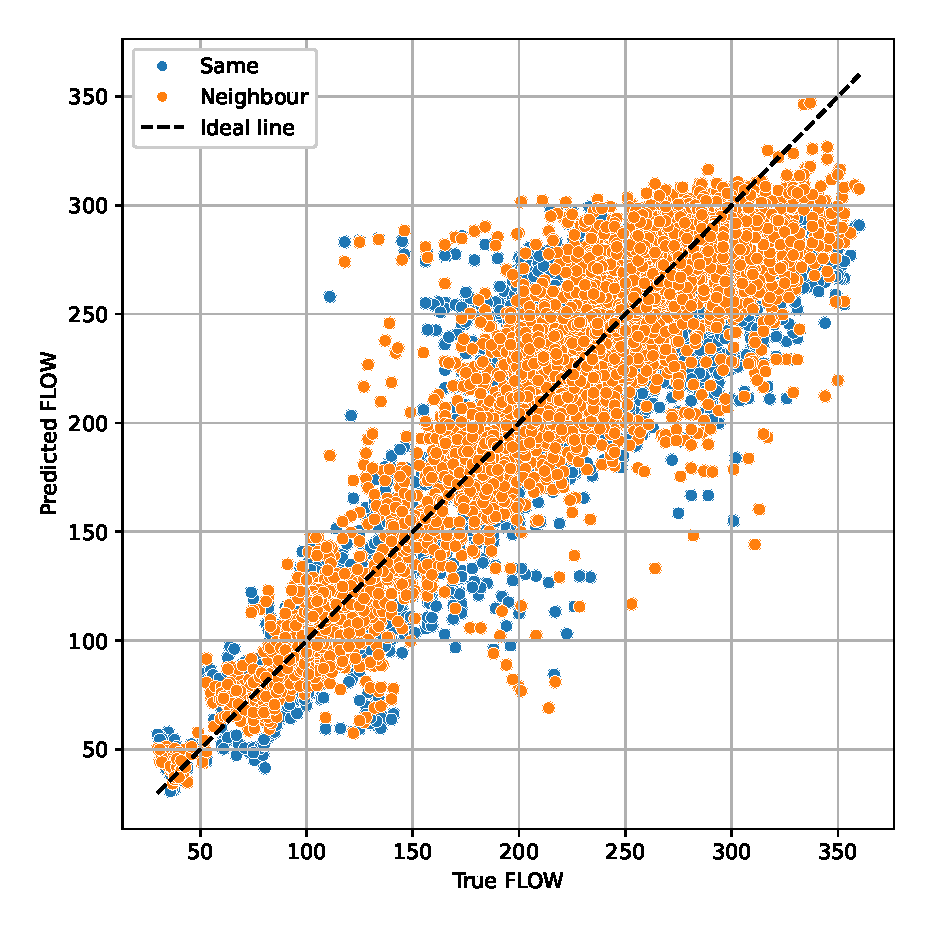
\includegraphics[width=\textwidth]{../Plots/Flow/samevsneighbour_nan}
			\caption{Flow: the orange (neighbour) points are  closer to the diagonal indicating better prediction from this sensor group}
		\end{subfigure}
		\begin{subfigure}{0.49 \linewidth}
			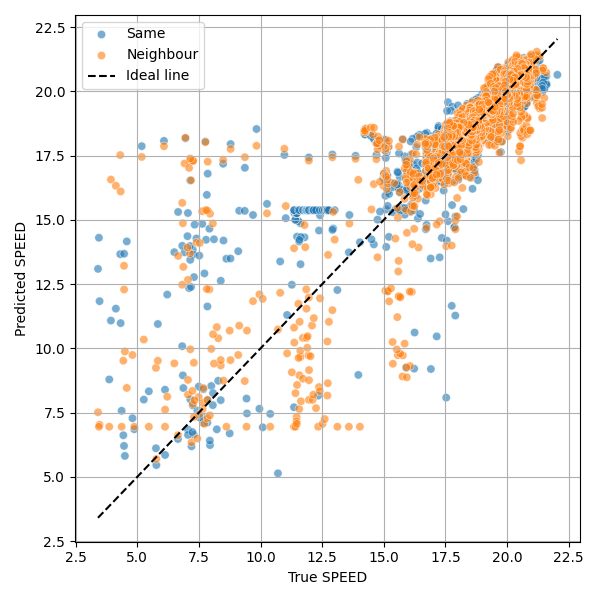
\includegraphics[width=\textwidth]{../Plots/Speed/samevsneighbour_nan}
			\caption{Speed: most of the values are predicted correctly, but the model has diffulties with predicting low speed values below 15 m/s}
		\end{subfigure}
		\caption{True vs predicted values}
		\label{fig:samevsneighbour_nan}
	\end{figure}
	\section{Model Deployment and Discussion}
	\subsection{Model Robustness }
	In this project, the robustnesss of each model was evaluated by applying it to unseen test data.  Furthermore, the XGBoost model was also evaluated on a separate evaluation set.
	A decline from the performance in the test set to the performance in the evaluation set was observed, however was relatively small.  The results suggest that the learned relationships between the target sensor and the neighbouring sensors are stable and can be applied to data outside the training period, demonstrating robustness in practical scenarios.
	\subsection{Handling Missing  Data}
	As explained in chapter \ref{chap:nan} with XGBoost as chosen model type, NaN-values can be handled internally in the predicting process. So, even if some data from a different sensor are missing, the flow and speed at the target value can still be predicted with a high accuracy. This makes this model type especially useful for real-time applications.
	\subsection{Practical Deployment Considerations}
	In a real-world deployment, a separate model could be trained for each target sensor using historical data from its neighbouring sensors. In case of a total sensor failure, the pre-trained model could then be used to predict the missing values in real time, ensuring continuity of traffic monitoring. This approach would allow the traffic management system to operate reliably even when individual sensors are offline. Additionally, models could be periodically retrained to adapt to changing traffic conditions.
	\subsection{Limitations and Future Work}
	The main limitation of this work is that all analyses and model evaluations were based on data from a single lane and portal. Consequently, the conclusions cannot yet be generalized to other locations or traffic conditions.
	In future work, additional sensors and portals should be included to evaluate spatial transferability.  \newline
	A further limitation is that the parameters of the XGBOOST model were tuned only once, and were not re-tuned for the third portal or for the model with NaN values.\newline  
	Furthermore, as already indicated in chapter \ref{chap:influencedistance} flow predictions based on data from the directly neighbouring portal performed better than those from the same or a more distant portal. This could indicate the existence of an optimal distance for capturing flow dynamics, which could also be investigated in a future work.
	
	\section{Conclusion}
	This study investigated different machine learning approaches for short-term traffic prediction based on sensor data from a single highway portal. Four models — Linear Regression, XGBoost, a Feedforward Neural Network, and an LSTM network — were developed and compared using RMSE, MAE and R² as performance metrics. Among these, XGBoost achieved the best overall results, combining high prediction results with computational efficiency. Furthermore, it was considered especially useful for real-life application as NaN-values can be handled internally. An external evaluation set was used to ensure that the model’s performance generalizes well to unseen data. \newline
	As answer to the initial research question, it was found that the speed could best be predicted by sensors in the same portal, while flow values could be better predicted with neighbouring sensors, partially refuting the initial hypothesis. On the evaluation set an R²-score of 0.803 was achieved for the flow and and R²-score of 0.739 was achieved for the speed, indicating that the model can be reliably used to predict missing sensor data from failing sensors. These results highlight the practical potential of such models to support traffic monitoring and management in real-time. Further work should extend the research to other target sensors, allowing for more general conclusions. It could also be considered to gradually reduce the number of sensors required, as not all of them appear to be necessary for monitoring traffic conditions, making the system more cost-effective.
	
	
	
	
	\newpage
	\appendix
	\section*{Appendix}
	\addcontentsline{toc}{section}{Appendix}
	\section{GitHub code link}
	The project can be accessed under:
	\url{https://github.com/Jojo18-20/Project_AI_Transportation}
	\section{Note on AI Assistance}
	ChatGPT was used as a supportive tool for debugging and for formulating parts of the code.
	\section{ Additional figures and tables}
		\begin{table}[H]
		\centering
		\caption{Portals and sensors}
		\label{tab:portalsandsensors}
		\begin{tabular}{|l|l|}
			\hline
			Portal & sensors \\
			\hline
			E4S 55620 & 751, 1254, 1076 \\
			E4S 56160 & 539, 536, 740 \\
			E4S 56490 & 351, 4873, 153, 902 \\
			E4S 56780 & 543, 534, 4872, 1079 \\
			E4S 57055 & 353, 1443, 749 \\
			E4S 57435 & 4430, 4429, 4437 \\
			E4S 57820 & 4427, 4436, 4428, 4439 \\
			E4S 58140 & 4494, 4473, 4495, 4472, 4496 \\
			\hline
		\end{tabular}
	\end{table}
	
	
		\begin{figure}[H]
		\centering
		\begin{subfigure}{0.49 \linewidth}
			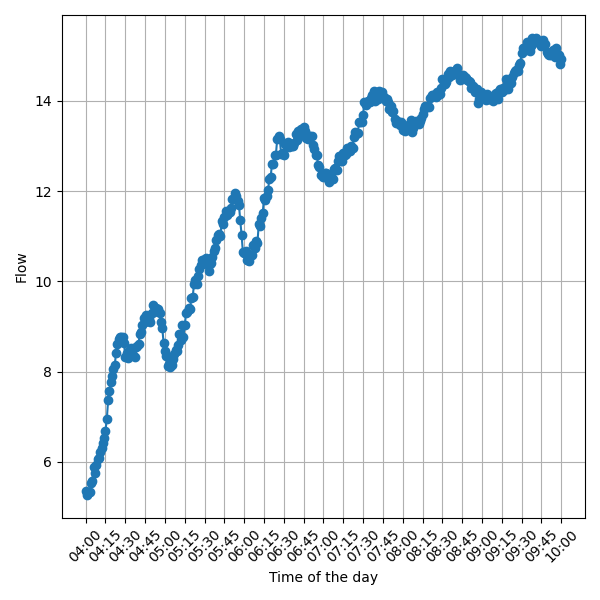
\includegraphics[width=\textwidth]{../Plots/Flow/avg_flow_day}
			\caption{Flow}
		\end{subfigure}
		\begin{subfigure}{0.49 \linewidth}
			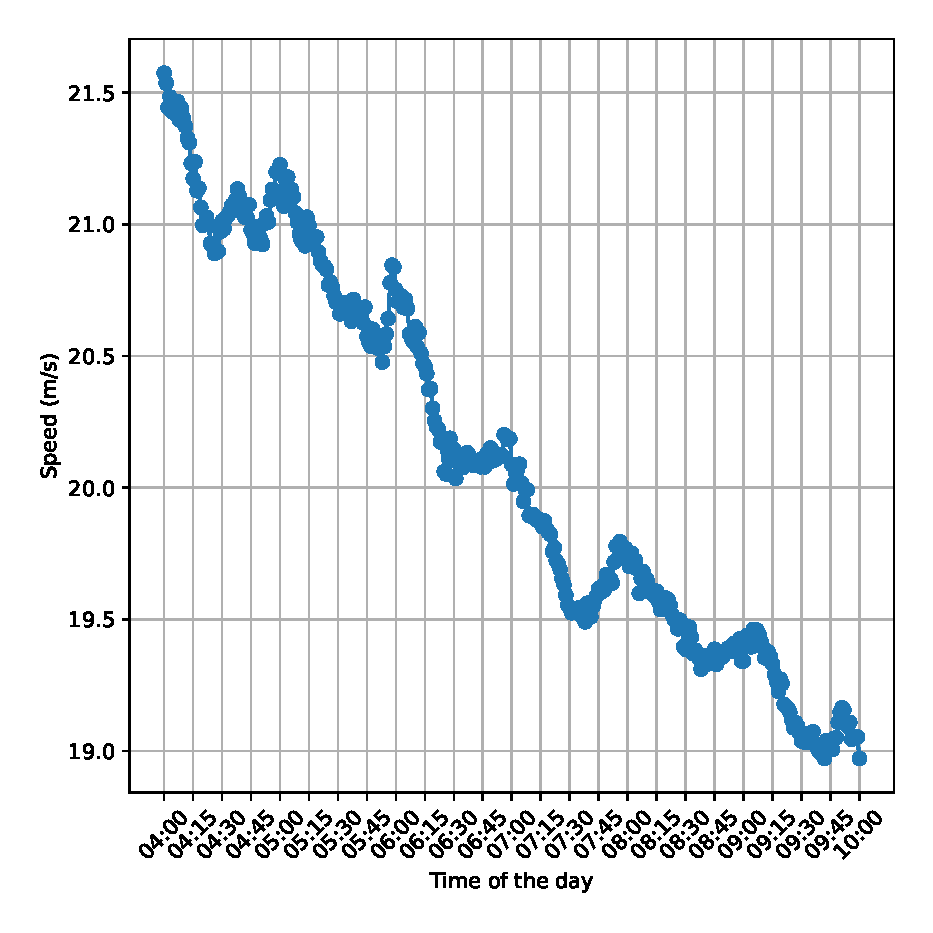
\includegraphics[width=\textwidth]{../Plots/Speed/avg_speed_day}
			\caption{Speed}
		\end{subfigure}
		\caption{Flow and Speed over the day}
		\label{fig:speed_and_flow_overday}
	\end{figure}
	\begin{figure}[H]
		\centering
		\begin{subfigure}{0.49 \linewidth}
			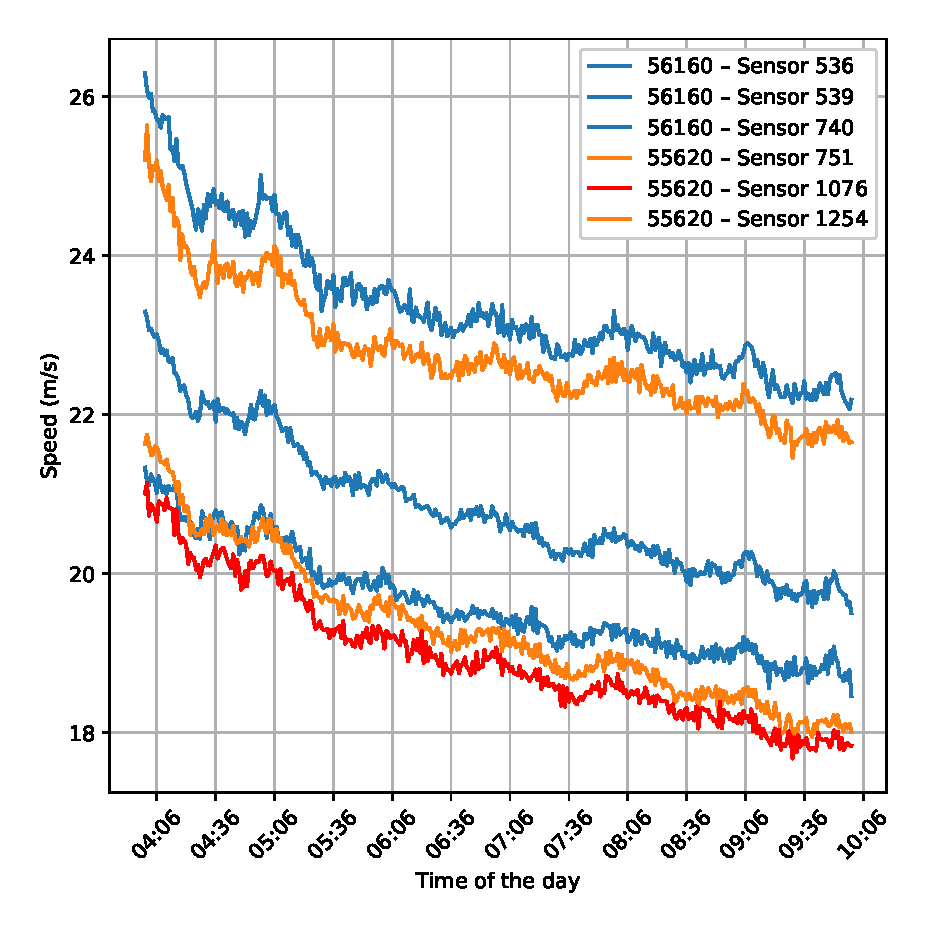
\includegraphics[width=\textwidth]{../Plots/Speed/avg_speed_day_per_sensor_portal}
			\caption{Flow}
		\end{subfigure}
		\begin{subfigure}{0.49 \linewidth}
			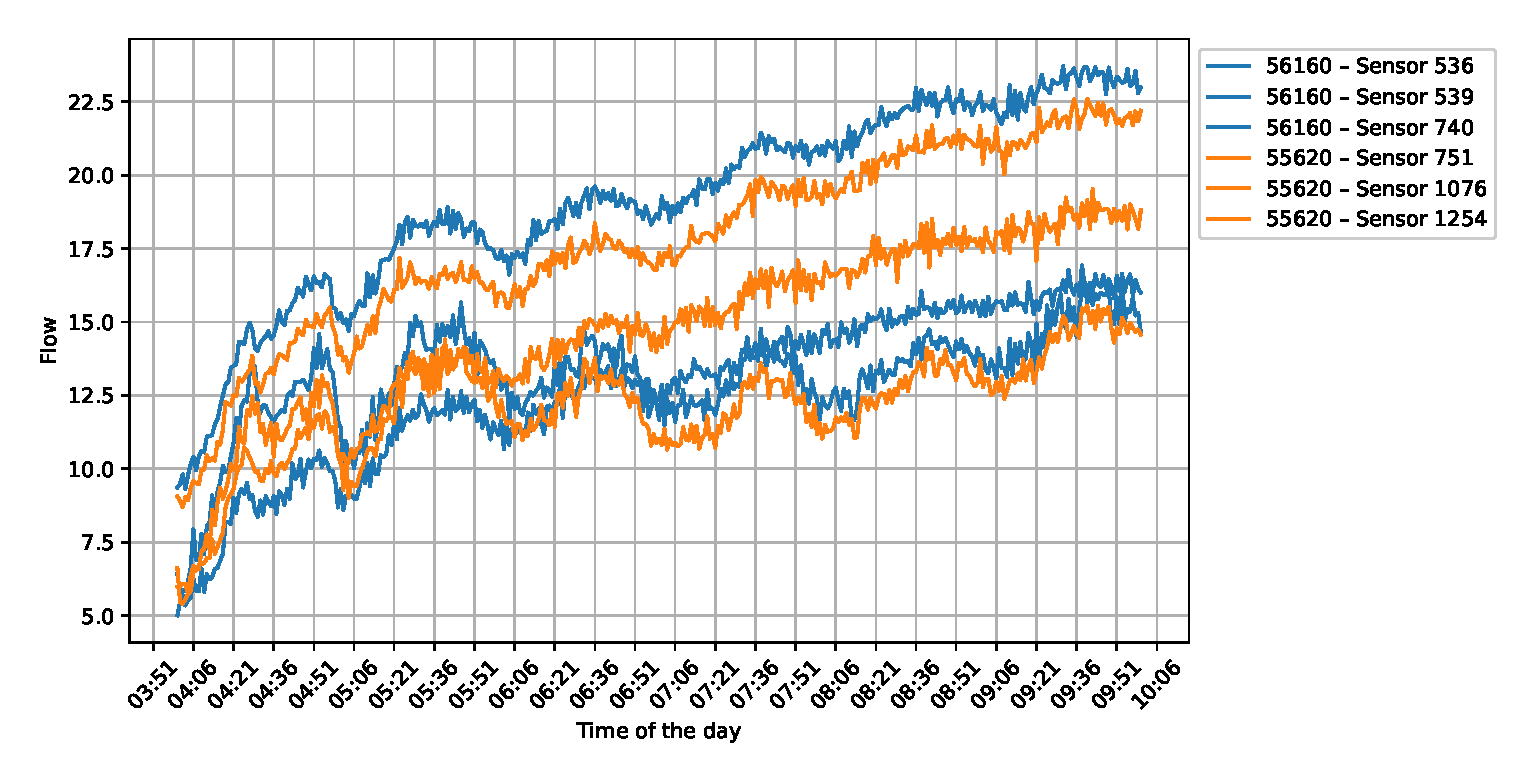
\includegraphics[width=\textwidth]{../Plots/Flow/avg_flow_day_per_sensor_portal}
			\caption{Speed}
		\end{subfigure}
		\caption{Flow and Speed for the sensors in portal 55620 and 56160: It can be seen that the pattern for sensors within the same portal can vary a lot, showing partially more similarity with the daily profil of sensors in other portals }
		\label{fig:speed_and_flow_sensors}
	\end{figure}

	\begin{figure}[H]
		\centering
		\begin{subfigure}{0.9 \linewidth}
			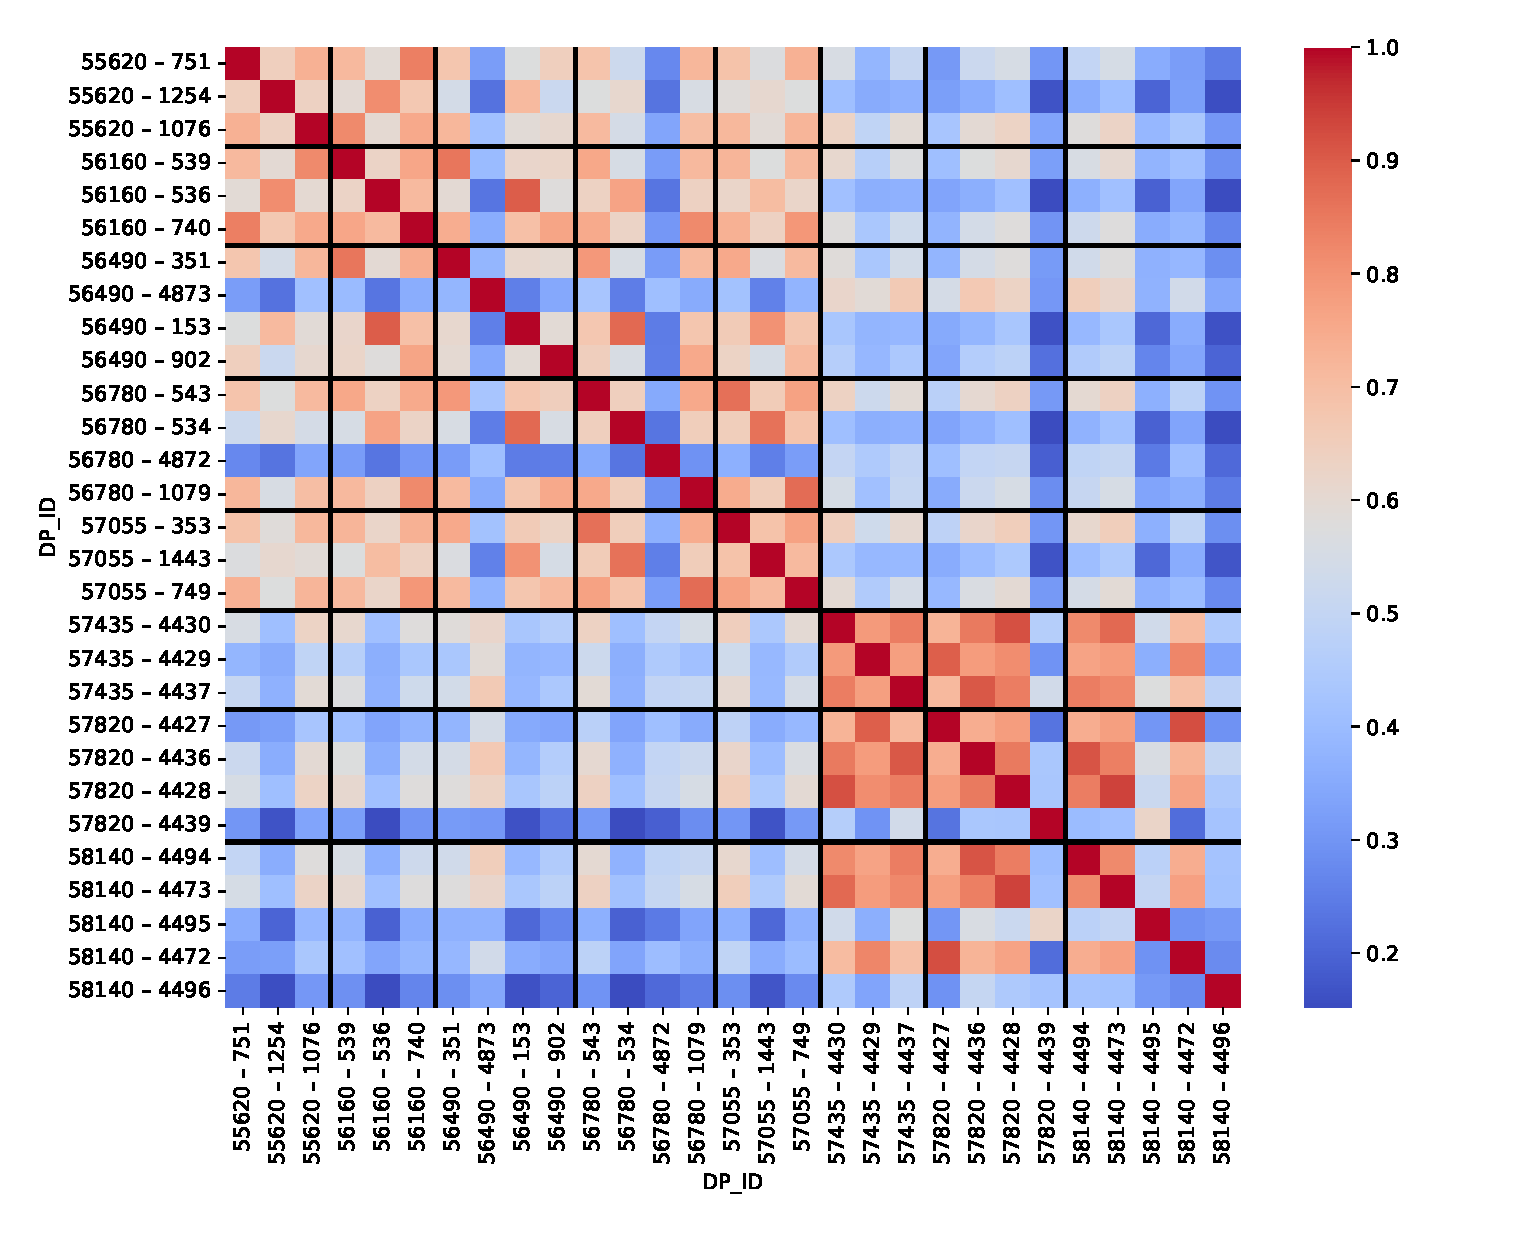
\includegraphics[width=\textwidth]{../Plots/Flow/sensor_corr_by_portal}
			\caption{Flow}
		\end{subfigure}
		\begin{subfigure}{0.9 \linewidth}
			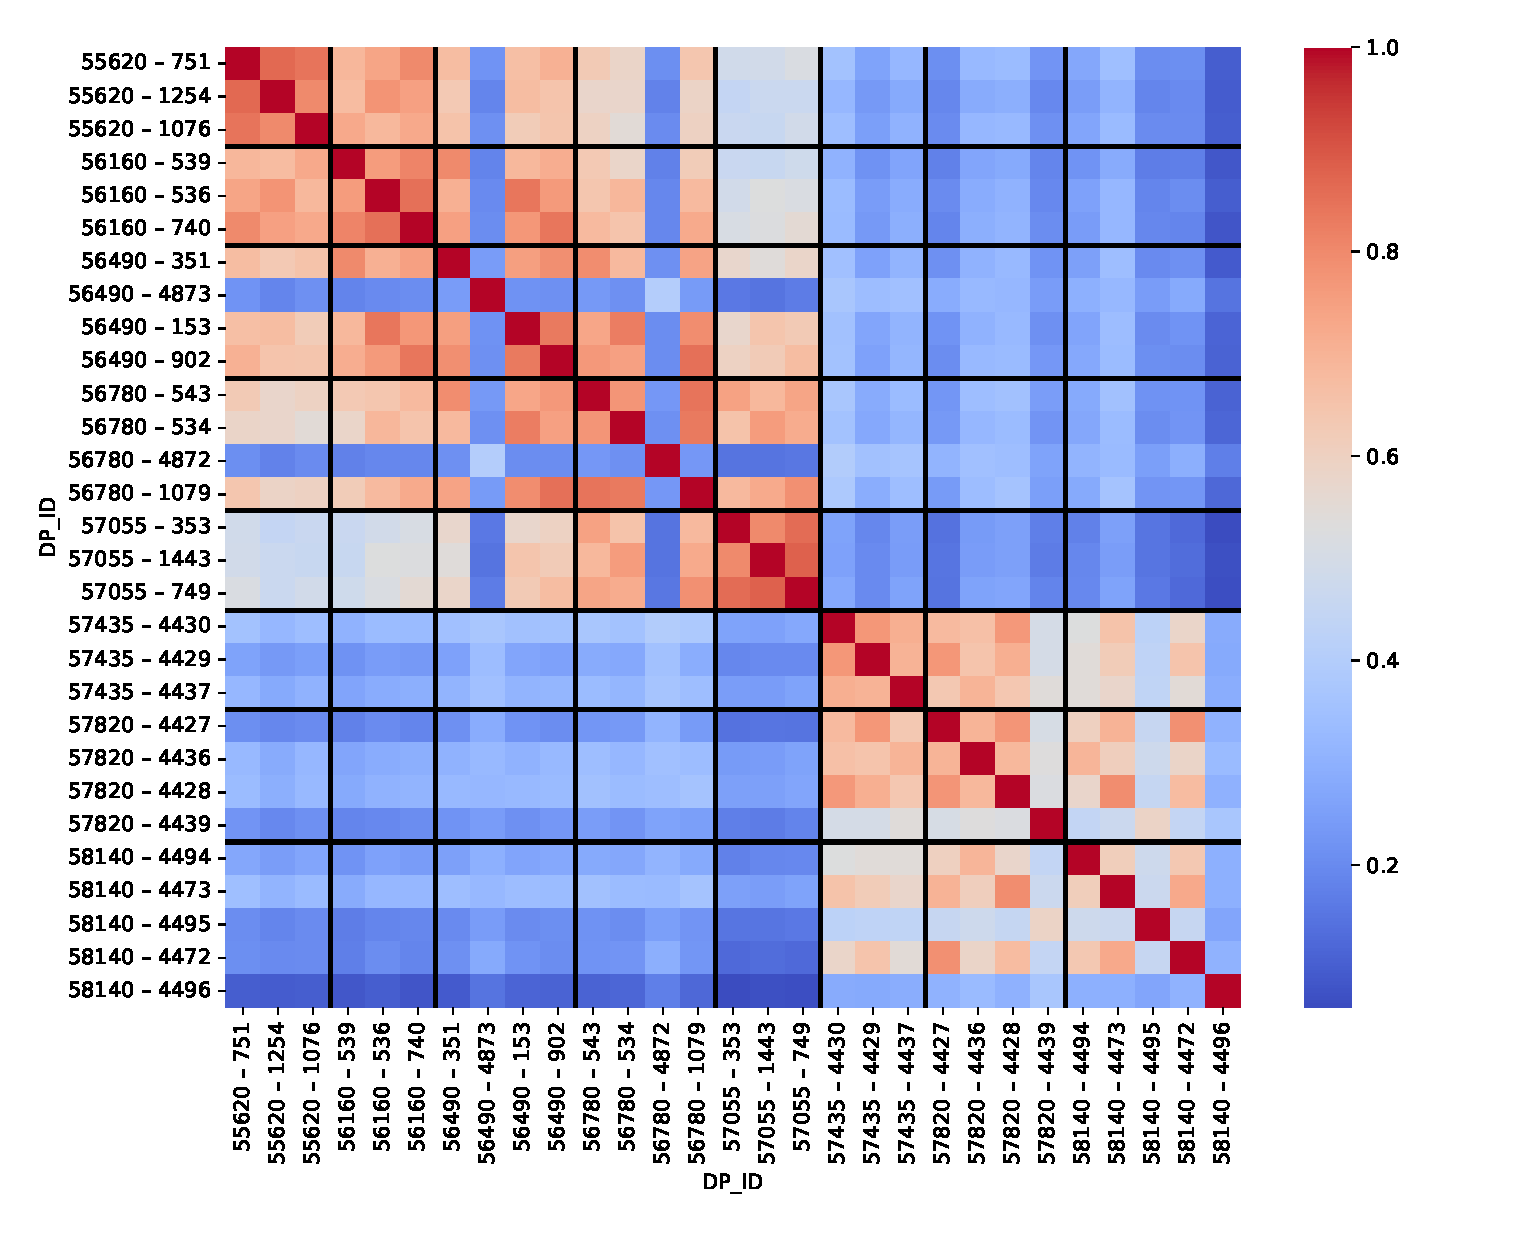
\includegraphics[width=\textwidth]{../Plots/Speed/sensor_corr_by_portal}
			\caption{Speed}
		\end{subfigure}
		\caption{Correlation between speed and flow in different sensors}
		\label{fig:sensor_corr_by_portal_big}
	\end{figure}
	\begin{table}[H]
		\centering
		\caption{The number and name of the sensor that belong to every cluster for every portal and the most likely lane that cluster corresponds to}
		\label{tab:cluster}
		\begin{tabular}{c|cccc}
			Portal/Cluster & 0 (exit/marging) & 1(left) & 2(middle) & 3 (right) \\
			\hline 
			55620          & 1 (1076)         & 0       & 1(1254)   & 1(751)    \\
			56160          & 1(539)           & 0       & 1(536)    & 1(740)    \\
			56490          & 1(351)           & 1(4873) & 1(153)    & 1(902)    \\
			56780          & 1(543)           & 1(4872) & 1(534)    & 1(1079)   \\
			57055          & 1(353)           & 0       & 1(1443)   & 1(749)   
		\end{tabular}
	\end{table}
	\begin{figure}[H]
		\centering
		\begin{subfigure}{0.49 \linewidth}
			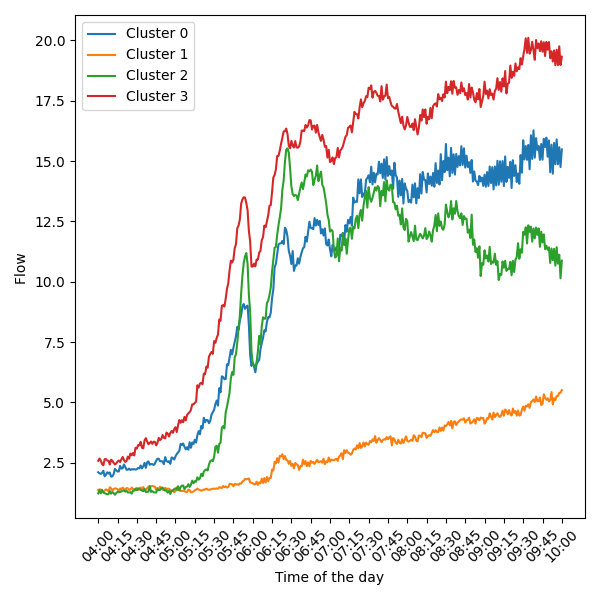
\includegraphics[width=\textwidth]{../Plots/Flow/clustering_3portals}
			\caption{Flow}
		\end{subfigure}
		\begin{subfigure}{0.49 \linewidth}
			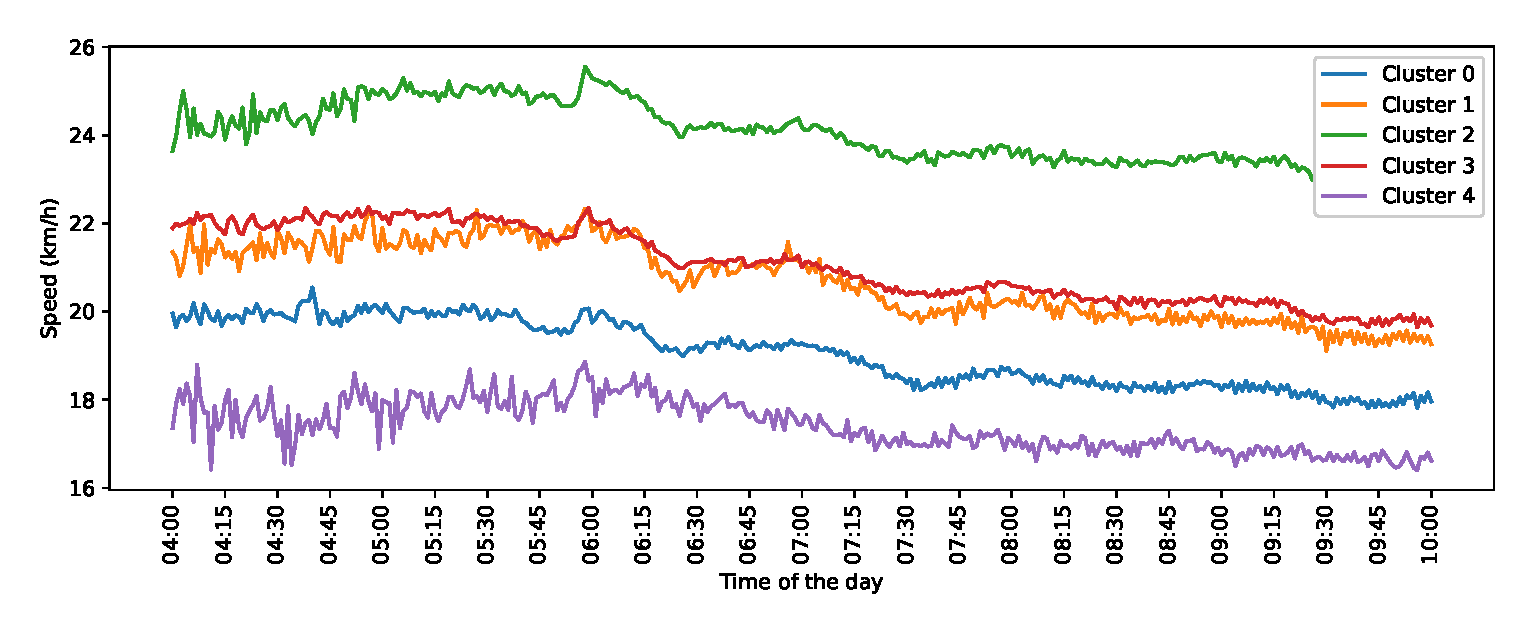
\includegraphics[width=\textwidth]{../Plots/Speed/clustering_3portals}
			\caption{Speed}
		\end{subfigure}
		\caption{Clustering for portals 58140, 57820 and 57435}
		\label{fig:clustering_3portals}
	\end{figure}
	\begin{figure}[H]
		\centering
		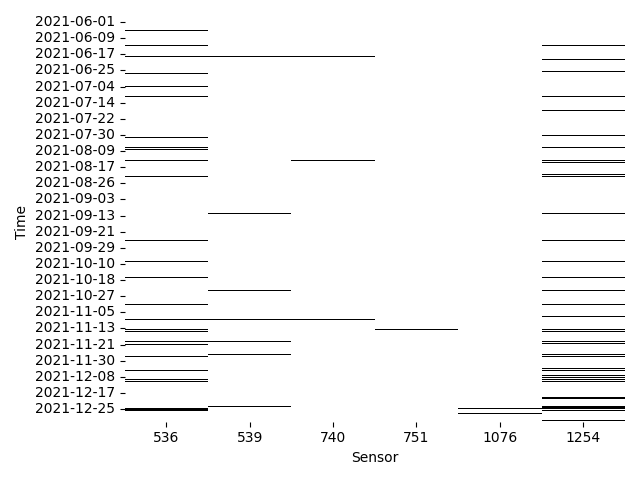
\includegraphics[width =0.5 \linewidth]{../Plots/missingvalues}
		\caption{Missing values}
		\label{fig:missingvalues}
	\end{figure}
	\begin{figure}[H]
		\centering
		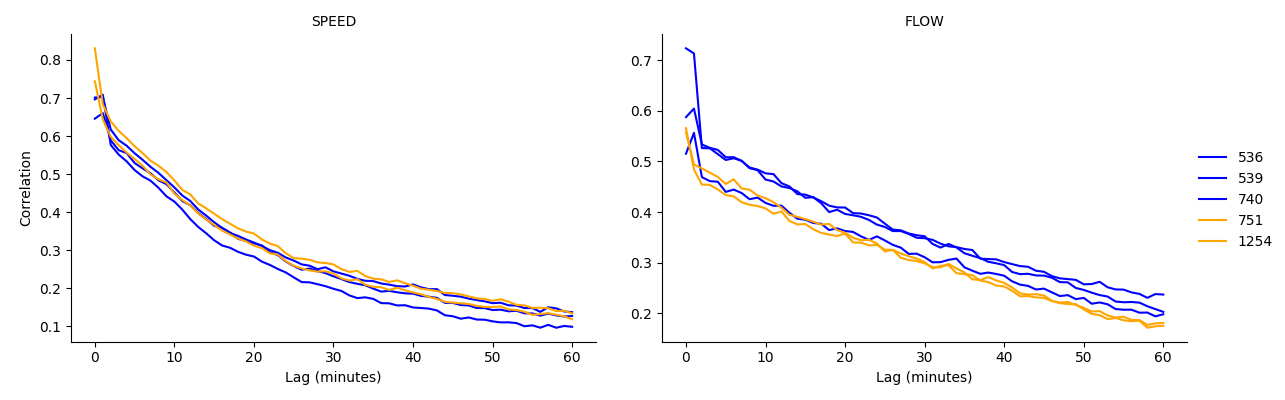
\includegraphics[width =0.99 \linewidth]{../Plots/Correlation_lag_flow_speed_peak}
		\caption{Correlation between the target value and the lagged valueso of the other sensors}
		\label{fig:correlation_lag}
	\end{figure}
	\begin{table}[H]
		\centering
		\caption{Results obtained with XGBoost on the evaluation set (filled dataset without Nan-values)}
		\label{tab:result_xgb_evaluation}
		\begin{tabular}{l|lll}
			& RMSE   & MAE    & R²    \\
			\hline
			Flow - same portal      &31.127 & 23.841 & 0.801\\
			Flow - neighbour portal &  27.295 &19.662 &0.847\\
			Speed - same portal     &1.029 & 0.475& 0.738\\
			Speed -neighbour portal & 1.173 & 0.533 & 0.659
		\end{tabular}
	\end{table}
		\begin{figure}[H]
		\centering
		\begin{subfigure}{0.49 \linewidth}
			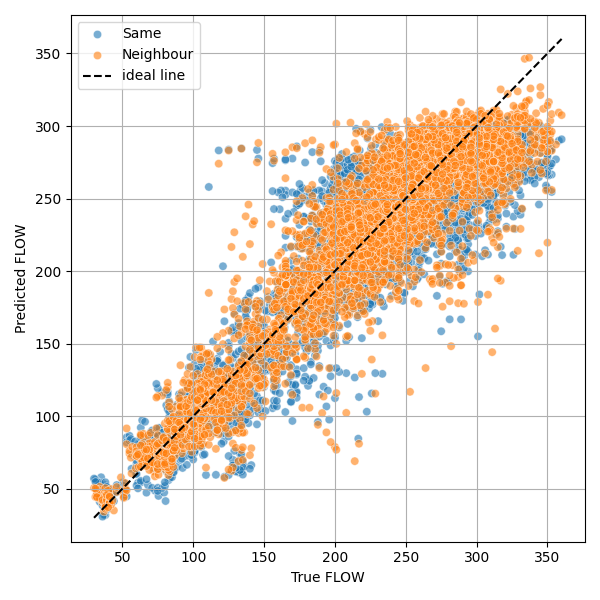
\includegraphics[width=\textwidth]{../Plots/Flow/samevsneighbour}
			\caption{Flow}
		\end{subfigure}
		\begin{subfigure}{0.49 \linewidth}
			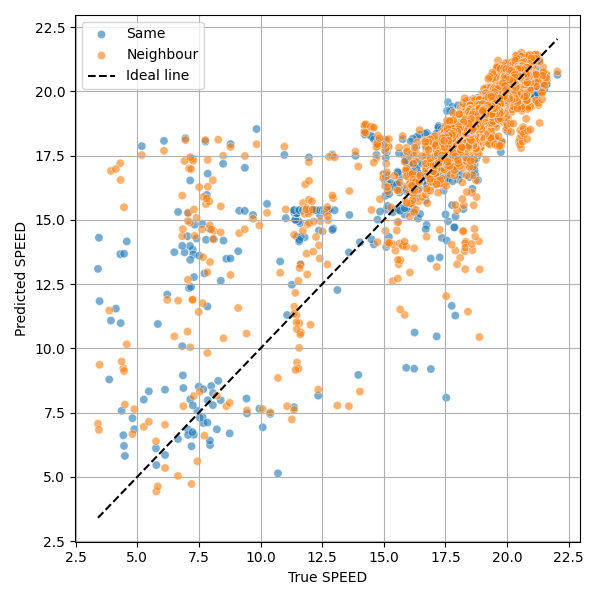
\includegraphics[width=\textwidth]{../Plots/Speed/samevsneighbour}
			\caption{Speed}
		\end{subfigure}
		\caption{True vs predicted values(filled dataset without Nan-values)}
		\label{fig:samevsneighbour}
	\end{figure}
	
	-------------------------------------------------------------------------%
	%------------------------------------------QUELLENVERZEICHNIS---------------------------------%
	%---------------------------------------------------------------------------------------------%
	%\newpage 
	
	\newpage
	\bibliography{literatur}
	%\bibliographystyle{babalpha}
	%\bibliographystyle{unsrt}
	\bibliographystyle{IEEEtran}
	
	%---------------------------------------------------------------------------------------------%
	%------------------------------------------ABBILDUNGSVERZEICHNIS------------------------------%
	%---------------------------------------------------------------------------------------------%
	%\listoffigures
	
	%---------------------------------------------------------------------------------------------%
	%------------------------------------------TABELLENVERZEICHNIS--------------------------------%
	%---------------------------------------------------------------------------------------------%
	%\listoftables
	
	%---------------------------------------------------------------------------------------------%
	%------------------------------------------ANHÄNGE--------------------------------------------%
	%---------------------------------------------------------------------------------------------%
	% Hier kann noch das Messprotokoll als eingescannte PDF angehängt werden 
	%\includepdf{dateiname}
	
	
\end{document}
